% =============================================================================
% Module 8.0: Network Operations and Monitoring
% Network+ Course - LaTeX Beamer Presentation
% Theme: Shrek
% =============================================================================

\documentclass[aspectratio=169, 11pt]{beamer}

% Theme and colors
\usetheme{Madrid}
\usecolortheme{default}

% Custom colors
\definecolor{rctcblue}{RGB}{0, 74, 136}
\definecolor{rctcgold}{RGB}{255, 199, 44}
\definecolor{networkgreen}{RGB}{0, 150, 100}
\definecolor{alertred}{RGB}{200, 50, 50}
\definecolor{aborange}{RGB}{230, 120, 0}
\definecolor{tcpblue}{RGB}{30, 100, 180}
\definecolor{udpgreen}{RGB}{50, 160, 80}
\definecolor{ogregreen}{RGB}{34, 139, 34}

% Set theme colors
\setbeamercolor{palette primary}{bg=rctcblue, fg=white}
\setbeamercolor{palette secondary}{bg=rctcblue!80, fg=white}
\setbeamercolor{palette tertiary}{bg=rctcblue!60, fg=white}
\setbeamercolor{structure}{fg=rctcblue}
\setbeamercolor{title}{fg=rctcblue}
\setbeamercolor{frametitle}{fg=rctcblue, bg=rctcblue!10}
\setbeamercolor{block title}{bg=rctcblue, fg=white}
\setbeamercolor{block body}{bg=rctcblue!5}
\setbeamercolor{block title alerted}{bg=alertred, fg=white}
\setbeamercolor{block body alerted}{bg=alertred!5}
\setbeamercolor{block title example}{bg=networkgreen, fg=white}
\setbeamercolor{block body example}{bg=networkgreen!5}

% Packages
\usepackage{tikz}
\usepackage{booktabs}
\usepackage{fontawesome5}
\usepackage{graphicx}
\usepackage{xcolor}
\usepackage{colortbl}
\usepackage{array}
\usepackage{listings}
\usepackage{amsmath}
\usepackage{amssymb}

% TikZ libraries
\usetikzlibrary{shapes.geometric, arrows.meta, positioning, decorations.pathreplacing, 
                backgrounds, fit, calc, shadows, shapes.symbols, shapes.misc}

% Connection styles
\tikzstyle{ethernet} = [draw, line width=1.5pt, color=rctcblue, -{Stealth}]
\tikzstyle{process} = [draw=rctcblue, fill=rctcblue!15, rounded corners,
                       minimum width=1.8cm, minimum height=0.5cm, font=\footnotesize, align=center]
\tikzstyle{decision} = [draw=aborange, fill=aborange!15, diamond, aspect=2,
                        minimum width=1.2cm, font=\footnotesize, align=center]

% Icon commands using FontAwesome
\newcommand{\iconpc}[1][0.6cm]{\resizebox{#1}{!}{\faIcon{desktop}}}
\newcommand{\iconlaptop}[1][0.6cm]{\resizebox{#1}{!}{\faIcon{laptop}}}
\newcommand{\iconserver}[1][0.6cm]{\resizebox{#1}{!}{\faIcon{server}}}
\newcommand{\iconrouter}[1][0.6cm]{\resizebox{#1}{!}{\faIcon{network-wired}}}
\newcommand{\iconswitch}[1][0.6cm]{\resizebox{#1}{!}{\faIcon{sitemap}}}
\newcommand{\iconfirewall}[1][0.6cm]{\resizebox{#1}{!}{\faIcon{shield-alt}}}
\newcommand{\iconcloud}[1][0.6cm]{\resizebox{#1}{!}{\faIcon{cloud}}}
\newcommand{\iconphone}[1][0.6cm]{\resizebox{#1}{!}{\faIcon{phone}}}
\newcommand{\icondatabase}[1][0.6cm]{\resizebox{#1}{!}{\faIcon{database}}}
\newcommand{\iconglobe}[1][0.6cm]{\resizebox{#1}{!}{\faIcon{globe}}}
\newcommand{\iconuser}[1][0.6cm]{\resizebox{#1}{!}{\faIcon{user}}}
\newcommand{\iconlock}[1][0.6cm]{\resizebox{#1}{!}{\faIcon{lock}}}
\newcommand{\iconclock}[1][0.6cm]{\resizebox{#1}{!}{\faIcon{clock}}}
\newcommand{\iconmail}[1][0.6cm]{\resizebox{#1}{!}{\faIcon{envelope}}}
\newcommand{\icondoc}[1][0.6cm]{\resizebox{#1}{!}{\faIcon{file-alt}}}
\newcommand{\iconsearch}[1][0.6cm]{\resizebox{#1}{!}{\faIcon{search}}}
\newcommand{\icontools}[1][0.6cm]{\resizebox{#1}{!}{\faIcon{tools}}}
\newcommand{\iconchart}[1][0.6cm]{\resizebox{#1}{!}{\faIcon{chart-line}}}
\newcommand{\iconalert}[1][0.6cm]{\resizebox{#1}{!}{\faIcon{bell}}}
\newcommand{\iconlog}[1][0.6cm]{\resizebox{#1}{!}{\faIcon{clipboard-list}}}
\newcommand{\iconeye}[1][0.6cm]{\resizebox{#1}{!}{\faIcon{eye}}}

% Listings style
\lstset{
    basicstyle=\ttfamily\scriptsize,
    breaklines=true,
    frame=single,
    backgroundcolor=\color{rctcblue!5},
    rulecolor=\color{rctcblue!50}
}

% Document info
\title[Module 8.0]{Module 8.0: Network Operations and Monitoring}
\subtitle{Network+ Certification Course}
\author{Brendan Shea, PhD}
\date{Introduction to Networking}
\institute{RCTC}

\begin{document}

% SLIDE 1: Title
\begin{frame}
    \titlepage
    \begin{center}
        \begin{tikzpicture}[scale=0.65]
            \node (monitor) at (0, 0) {\iconserver[0.5cm]};
            \node[font=\tiny, below=0.05cm of monitor] {NMS};
            \node (r1) at (-2.5, 1.5) {\iconrouter[0.4cm]};
            \node (sw1) at (0, 2) {\iconswitch[0.4cm]};
            \node (s1) at (2.5, 1.5) {\iconserver[0.4cm]};
            \draw[dashed, ogregreen, -{Stealth}] (monitor) -- (r1);
            \draw[dashed, ogregreen, -{Stealth}] (monitor) -- (sw1);
            \draw[dashed, ogregreen, -{Stealth}] (monitor) -- (s1);
        \end{tikzpicture}
    \end{center}
\end{frame}

% SLIDE 2: Module Overview
\begin{frame}{Module 8 Learning Objectives}
    \begin{columns}[T]
        \begin{column}{0.48\textwidth}
            \begin{block}{1. Documentation \& Policies}
                \footnotesize
                \begin{itemize}\setlength{\itemsep}{0pt}
                    \item Configuration management
                    \item Change management processes
                    \item Physical \& logical diagrams
                    \item Asset and lifecycle management
                \end{itemize}
            \end{block}
            \begin{block}{2. Discovery \& Monitoring}
                \footnotesize
                \begin{itemize}\setlength{\itemsep}{0pt}
                    \item Network discovery (nmap)
                    \item Performance monitoring
                    \item Availability and configuration checks
                \end{itemize}
            \end{block}
        \end{column}
        \begin{column}{0.48\textwidth}
            \begin{block}{3. SNMP \& Event Management}
                \footnotesize
                \begin{itemize}\setlength{\itemsep}{0pt}
                    \item SNMP agents, versions, security
                    \item Syslog and centralized logging
                    \item SIEM and event correlation
                \end{itemize}
            \end{block}
            \begin{block}{4. Traffic Analysis}
                \footnotesize
                \begin{itemize}\setlength{\itemsep}{0pt}
                    \item Packet capture (tcpdump, Wireshark)
                    \item Flow data (NetFlow, sFlow)
                    \item QoS and traffic shaping
                \end{itemize}
            \end{block}
        \end{column}
    \end{columns}
\end{frame}

% SLIDE 3: Why Documentation Matters
\begin{frame}{Section 8.1: Why Documentation Matters}
    \begin{columns}[T]
        \begin{column}{0.48\textwidth}
            \begin{block}{The Swamp Network Problem}
                \footnotesize
                Without documentation, networks become \textbf{unmaintainable swamps}:
                \begin{itemize}\setlength{\itemsep}{0pt}
                    \item No one knows what's connected where
                    \item Changes break unknown dependencies
                    \item Troubleshooting takes hours instead of minutes
                    \item New staff can't understand the environment
                \end{itemize}
            \end{block}
            \begin{alertblock}{Key Takeaway}
                \footnotesize
                Good documentation is the difference between a \textbf{manageable network} and a \textbf{chaotic swamp}!
            \end{alertblock}
        \end{column}
        \begin{column}{0.48\textwidth}
            \begin{center}
                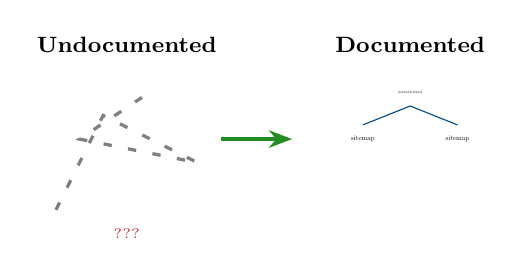
\begin{tikzpicture}[scale=0.6]
                    \node[font=\footnotesize] at (-2, 3) {\textbf{Undocumented}};
                    \draw[gray, very thick, loosely dashed] (-3.5, -0.5) -- (-2.5, 1.5) -- (-0.5, 0.5) -- (-3, 1) -- (-1.5, 2);
                    \node[font=\tiny, alertred] at (-2, -1) {???};
                    \draw[-{Stealth}, very thick, ogregreen] (0, 1) -- (1.5, 1);
                    \node[font=\footnotesize] at (4, 3) {\textbf{Documented}};
                    \node at (4, 2) {\iconrouter[0.3cm]};
                    \node at (3, 1) {\iconswitch[0.3cm]};
                    \node at (5, 1) {\iconswitch[0.3cm]};
                    \draw[rctcblue] (4,1.7) -- (3,1.3);
                    \draw[rctcblue] (4,1.7) -- (5,1.3);
                \end{tikzpicture}
            \end{center}
            \begin{exampleblock}{Documentation Types}
                \footnotesize
                Configuration management, change management, asset inventory, network diagrams, IPAM
            \end{exampleblock}
        \end{column}
    \end{columns}
\end{frame}

% SLIDE 4: Configuration Management
\begin{frame}{Configuration Management}
    \begin{columns}[T]
        \begin{column}{0.48\textwidth}
            \begin{block}{What is Configuration Management?}
                \footnotesize
                The practice of maintaining \textbf{consistent, documented device configurations} across your network infrastructure.
                \begin{itemize}\setlength{\itemsep}{0pt}
                    \item Baseline configurations (templates)
                    \item Version control for changes
                    \item Automated compliance checking
                    \item Rollback capabilities
                \end{itemize}
            \end{block}
            \begin{alertblock}{Why It Matters}
                \footnotesize
                Configuration drift causes outages! Consistent configs mean predictable behavior.
            \end{alertblock}
        \end{column}
        \begin{column}{0.48\textwidth}
            \begin{block}{Configuration Management Elements}
                \footnotesize
                \begin{tabular}{@{}l l@{}}
                    \toprule
                    \textbf{Element} & \textbf{Purpose} \\
                    \midrule
                    Baseline & Standard reference \\
                    Version Control & Track all changes \\
                    Validation & Check compliance \\
                    Backup & Enable recovery \\
                    Templates & Consistent deploys \\
                    \bottomrule
                \end{tabular}
            \end{block}
            \begin{exampleblock}{Common Tools}
                \footnotesize
                \textbf{RANCID}, \textbf{Oxidized}, SolarWinds NCM, Ansible, Git for network configs
            \end{exampleblock}
        \end{column}
    \end{columns}
\end{frame}

% SLIDE 5: Network Device Backup Management
\begin{frame}{Network Device Backup Management}
    \begin{columns}[T]
        \begin{column}{0.48\textwidth}
            \begin{block}{What to Backup}
                \footnotesize
                \begin{itemize}\setlength{\itemsep}{1pt}
                    \item \textbf{Startup-config}: Saved configuration
                    \item \textbf{Running-config}: Active configuration
                    \item \textbf{Firmware/IOS images}: Operating system
                    \item \textbf{Certificates \& keys}: Security material
                    \item \textbf{License files}: Entitlements
                \end{itemize}
            \end{block}
            \begin{alertblock}{The 3-2-1 Rule}
                \footnotesize
                \textbf{3} copies of data, on \textbf{2} different media types, with \textbf{1} copy offsite
            \end{alertblock}
        \end{column}
        \begin{column}{0.48\textwidth}
            \begin{center}
                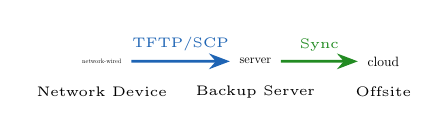
\begin{tikzpicture}[scale=0.65]
                    \node (device) at (0, 2) {\iconrouter[0.5cm]};
                    \node[font=\tiny] at (0, 1.4) {Network Device};
                    \node (backup) at (3, 2) {\iconserver[0.4cm]};
                    \node[font=\tiny] at (3, 1.4) {Backup Server};
                    \node (cloud) at (5.5, 2) {\iconcloud[0.4cm]};
                    \node[font=\tiny] at (5.5, 1.4) {Offsite};
                    \draw[-{Stealth}, tcpblue, line width=1pt] (device) -- (backup) node[midway, above, font=\tiny] {TFTP/SCP};
                    \draw[-{Stealth}, ogregreen, line width=1pt] (backup) -- (cloud) node[midway, above, font=\tiny] {Sync};
                \end{tikzpicture}
            \end{center}
            \begin{block}{Backup Schedule}
                \footnotesize
                \begin{tabular}{@{}l l@{}}
                    \toprule
                    \textbf{Frequency} & \textbf{What} \\
                    \midrule
                    On change & Running-config \\
                    Daily & All configs \\
                    Weekly & Firmware images \\
                    \bottomrule
                \end{tabular}
            \end{block}
        \end{column}
    \end{columns}
\end{frame}

% SLIDE 6: Change Management Process
\begin{frame}{Change Management Process}
    \begin{columns}[T]
        \begin{column}{0.55\textwidth}
            \begin{center}
                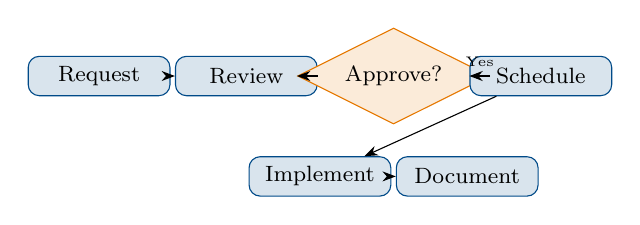
\begin{tikzpicture}[scale=0.85, node distance=1cm]
                    \node[process] (req) at (0, 0) {Request};
                    \node[process] (rev) at (2.2, 0) {Review};
                    \node[decision] (app) at (4.4, 0) {Approve?};
                    \node[process] (sched) at (6.6, 0) {Schedule};
                    \node[process] (impl) at (3.3, -1.5) {Implement};
                    \node[process] (doc) at (5.5, -1.5) {Document};
                    \draw[-{Stealth}] (req) -- (rev);
                    \draw[-{Stealth}] (rev) -- (app);
                    \draw[-{Stealth}] (app) -- node[above, font=\tiny] {Yes} (sched);
                    \draw[-{Stealth}] (sched) -- (impl);
                    \draw[-{Stealth}] (impl) -- (doc);
                \end{tikzpicture}
            \end{center}
            \begin{block}{Change Types}
                \footnotesize
                \begin{tabular}{@{}l l l@{}}
                    \toprule
                    \textbf{Type} & \textbf{Example} & \textbf{Approval} \\
                    \midrule
                    Standard & Password reset & Pre-approved \\
                    Normal & VLAN addition & CAB review \\
                    Emergency & Security patch & Expedited \\
                    \bottomrule
                \end{tabular}
            \end{block}
        \end{column}
        \begin{column}{0.42\textwidth}
            \begin{block}{CAB = Change Advisory Board}
                \footnotesize
                Team that reviews and approves changes:
                \begin{itemize}\setlength{\itemsep}{0pt}
                    \item Assesses risk and impact
                    \item Schedules maintenance windows
                    \item Ensures rollback plans exist
                \end{itemize}
            \end{block}
            \begin{alertblock}{Key Principle}
                \footnotesize
                \textbf{No undocumented changes!} Every change needs a ticket, approval, and verification.
            \end{alertblock}
        \end{column}
    \end{columns}
\end{frame}

% SLIDE 7: Case Study - Donkey's Unauthorized Change
\begin{frame}{Case Study: Donkey's Unauthorized Network Change}
    \begin{alertblock}{``I'm Making Waffles... and WiFi!''}
        \footnotesize
        Donkey decides to ``help'' by adding a rogue wireless access point to the Swamp Castle network so visitors can connect more easily. He plugs it directly into a core switch port.
        
        \vspace{0.2em}
        The next morning, Lord Farquaad's security team detects multiple unknown devices on the network. Investigation reveals the unsecured AP has been broadcasting ``SwampCastle-Guest'' with no password, and several unauthorized users have connected---including someone running network scans.
        
        \vspace{0.2em}
        \textbf{Current situation:} Rogue AP on VLAN 1 (management VLAN), no encryption, unknown devices accessing internal resources.
    \end{alertblock}
    \begin{block}{Review Questions}
        \footnotesize
        \begin{enumerate}\setlength{\itemsep}{0pt}
            \item What change management steps did Donkey skip?
            \item What documentation should exist for wireless additions?
            \item How could this security breach have been prevented?
        \end{enumerate}
    \end{block}
\end{frame}

% SLIDE 8: Case Study Solution - Donkey's Change
\begin{frame}{Case Study Solution: Donkey's Unauthorized Change}
    \begin{exampleblock}{Solution: ``That'll Do, Donkey---After Proper Approval!''}
        \footnotesize
        \begin{enumerate}\setlength{\itemsep}{1pt}
            \item Donkey skipped \textbf{all} steps: no request, no review, no approval, no documentation
            \item Required docs: Change request, security review, network diagram update, IPAM entry
            \item Prevention: \textbf{Port security}, \textbf{802.1X}, \textbf{change management policy training}
        \end{enumerate}
    \end{exampleblock}
    \begin{columns}[T]
        \begin{column}{0.48\textwidth}
            \begin{center}
                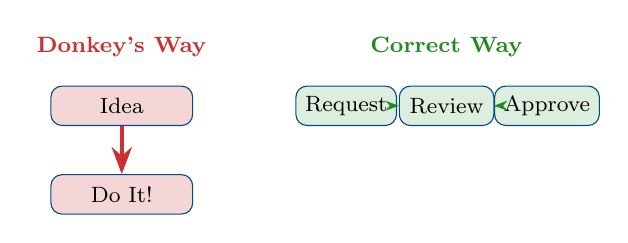
\begin{tikzpicture}[scale=0.75]
                    \node[font=\footnotesize, alertred] at (0, 3) {\textbf{Donkey's Way}};
                    \node[process, fill=alertred!20] (idea) at (0, 2) {Idea};
                    \node[process, fill=alertred!20] (do) at (0, 0.5) {Do It!};
                    \draw[-{Stealth}, alertred, line width=1.5pt] (idea) -- (do);
                    \node[font=\footnotesize, ogregreen] at (5.5, 3) {\textbf{Correct Way}};
                    \node[process, fill=ogregreen!15, minimum width=1.2cm] (r) at (3.8, 2) {Request};
                    \node[process, fill=ogregreen!15, minimum width=1.2cm] (a) at (5.5, 2) {Review};
                    \node[process, fill=ogregreen!15, minimum width=1.2cm] (d) at (7.2, 2) {Approve};
                    \draw[-{Stealth}, ogregreen] (r) -- (a);
                    \draw[-{Stealth}, ogregreen] (a) -- (d);
                \end{tikzpicture}
            \end{center}
        \end{column}
        \begin{column}{0.48\textwidth}
            \begin{alertblock}{Key Lesson}
                \footnotesize
                Even \textbf{helpful} changes can cause security breaches. Change management exists to protect the network---not to slow people down!
            \end{alertblock}
        \end{column}
    \end{columns}
\end{frame}

% SLIDE 9: Asset Inventory Documentation
\begin{frame}{Asset Inventory Documentation}
    \begin{columns}[T]
        \begin{column}{0.48\textwidth}
            \begin{block}{What to Track}
                \footnotesize
                \begin{itemize}\setlength{\itemsep}{1pt}
                    \item \textbf{Hardware}: Routers, switches, servers, APs
                    \item \textbf{Software}: OS versions, licenses, patches
                    \item \textbf{Location}: Rack, room, building, site
                    \item \textbf{Ownership}: Department, cost center
                    \item \textbf{Lifecycle}: Purchase, warranty, EOL dates
                \end{itemize}
            \end{block}
            \begin{alertblock}{Why Track Assets?}
                \footnotesize
                Security (know what's on network), compliance (license audits), planning (budget/refresh), troubleshooting
            \end{alertblock}
        \end{column}
        \begin{column}{0.48\textwidth}
            \begin{block}{Asset Inventory Fields}
                \footnotesize
                \begin{tabular}{@{}l l@{}}
                    \toprule
                    \textbf{Field} & \textbf{Example} \\
                    \midrule
                    Asset Tag & SW-CORE-001 \\
                    Hostname & swamp-sw-01 \\
                    Serial Number & FTX1234ABCD \\
                    MAC Address & AA:BB:CC:DD:EE:FF \\
                    IP Address & 10.1.1.2 \\
                    Location & Swamp DC, Rack 3 \\
                    Purchase Date & 2024-01-15 \\
                    \bottomrule
                \end{tabular}
            \end{block}
        \end{column}
    \end{columns}
\end{frame}

% SLIDE 10: Lifecycle Management
\begin{frame}{Lifecycle Management \& Decommissioning}
    \begin{columns}[T]
        \begin{column}{0.55\textwidth}
            \begin{center}
                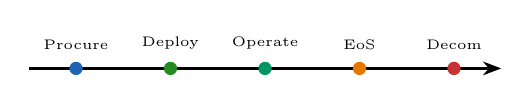
\begin{tikzpicture}[scale=0.6]
                    \draw[-{Stealth}, thick] (0, 0) -- (10, 0);
                    \fill[tcpblue] (1, 0) circle (4pt);
                    \node[font=\tiny, above] at (1, 0.2) {Procure};
                    \fill[ogregreen] (3, 0) circle (4pt);
                    \node[font=\tiny, above] at (3, 0.2) {Deploy};
                    \fill[networkgreen] (5, 0) circle (4pt);
                    \node[font=\tiny, above] at (5, 0.2) {Operate};
                    \fill[aborange] (7, 0) circle (4pt);
                    \node[font=\tiny, above] at (7, 0.2) {EoS};
                    \fill[alertred] (9, 0) circle (4pt);
                    \node[font=\tiny, above] at (9, 0.2) {Decom};
                \end{tikzpicture}
            \end{center}
            \begin{block}{Key Lifecycle Terms}
                \footnotesize
                \begin{itemize}\setlength{\itemsep}{0pt}
                    \item \textbf{EoS} (End of Sale): No longer sold
                    \item \textbf{EoSW} (End of Software): No new features
                    \item \textbf{EoL} (End of Life): No support/patches
                    \item \textbf{Decommission}: Proper removal
                \end{itemize}
            \end{block}
        \end{column}
        \begin{column}{0.42\textwidth}
            \begin{block}{Decommissioning Checklist}
                \footnotesize
                \begin{enumerate}\setlength{\itemsep}{0pt}
                    \item Backup final configuration
                    \item Document current connections
                    \item Notify affected users
                    \item \textbf{Wipe all data securely}
                    \item Revoke certificates/keys
                    \item Update inventory/diagrams
                \end{enumerate}
            \end{block}
            \begin{alertblock}{Security Warning}
                \footnotesize
                Old devices contain configs, credentials, and keys. \textbf{Always sanitize before disposal!}
            \end{alertblock}
        \end{column}
    \end{columns}
\end{frame}

% SLIDE 11: Physical Network Diagrams
\begin{frame}{Physical Network Diagrams}
    \begin{columns}[T]
        \begin{column}{0.48\textwidth}
            \begin{block}{What Physical Diagrams Show}
                \footnotesize
                \begin{itemize}\setlength{\itemsep}{1pt}
                    \item \textbf{Actual device locations} (racks, rooms)
                    \item \textbf{Cable runs} with labels and types
                    \item \textbf{Port assignments} (Gi0/1 to Patch 24)
                    \item \textbf{Rack elevations} and power connections
                    \item Physical redundancy paths
                \end{itemize}
            \end{block}
            \begin{exampleblock}{Use Cases}
                \footnotesize
                Technician dispatches, cable tracing, capacity planning, disaster recovery
            \end{exampleblock}
        \end{column}
        \begin{column}{0.48\textwidth}
            \begin{center}
                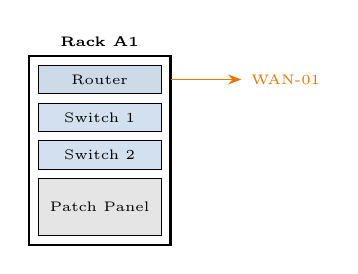
\begin{tikzpicture}[scale=0.6]
                    \draw[thick] (0, 0) rectangle (3, 4);
                    \node[font=\tiny] at (1.5, 4.3) {\textbf{Rack A1}};
                    \draw[fill=rctcblue!20] (0.2, 3.2) rectangle (2.8, 3.8);
                    \node[font=\tiny] at (1.5, 3.5) {Router};
                    \draw[fill=tcpblue!20] (0.2, 2.4) rectangle (2.8, 3);
                    \node[font=\tiny] at (1.5, 2.7) {Switch 1};
                    \draw[fill=tcpblue!20] (0.2, 1.6) rectangle (2.8, 2.2);
                    \node[font=\tiny] at (1.5, 1.9) {Switch 2};
                    \draw[fill=gray!20] (0.2, 0.2) rectangle (2.8, 1.4);
                    \node[font=\tiny] at (1.5, 0.8) {Patch Panel};
                    \draw[-{Stealth}, aborange] (3, 3.5) -- (4.5, 3.5) node[right, font=\tiny] {WAN-01};
                \end{tikzpicture}
            \end{center}
            \begin{block}{Diagram Elements}
                \footnotesize
                Device icons, cable lines, port labels, physical location markers
            \end{block}
        \end{column}
    \end{columns}
\end{frame}

% SLIDE 12: Logical Network Diagrams
\begin{frame}{Logical Network Diagrams}
    \begin{columns}[T]
        \begin{column}{0.48\textwidth}
            \begin{block}{What Logical Diagrams Show}
                \footnotesize
                \begin{itemize}\setlength{\itemsep}{1pt}
                    \item \textbf{IP addressing} and subnets
                    \item \textbf{VLAN assignments}
                    \item \textbf{Routing relationships}
                    \item \textbf{Logical groupings} (not physical)
                    \item Layer 3 topology
                \end{itemize}
            \end{block}
            \begin{block}{Physical vs Logical}
                \footnotesize
                \begin{tabular}{@{}l l@{}}
                    \toprule
                    \textbf{Physical} & \textbf{Logical} \\
                    \midrule
                    Where things are & How things connect \\
                    Cable paths & IP subnets \\
                    Rack locations & VLAN boundaries \\
                    \bottomrule
                \end{tabular}
            \end{block}
        \end{column}
        \begin{column}{0.48\textwidth}
            \begin{center}
                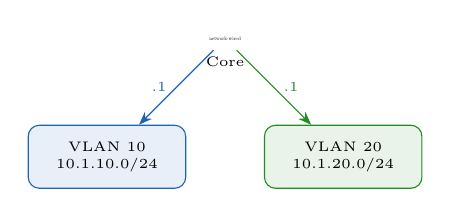
\begin{tikzpicture}[scale=0.6]
                    \node (core) at (2.5, 3) {\iconrouter[0.4cm]};
                    \node[font=\tiny] at (2.5, 2.5) {Core};
                    \node[draw=tcpblue, fill=tcpblue!10, rounded corners, 
                          minimum width=2cm, minimum height=0.8cm, font=\tiny, align=center] 
                          (vlan10) at (0, 0.5) {VLAN 10\\10.1.10.0/24};
                    \node[draw=ogregreen, fill=ogregreen!10, rounded corners, 
                          minimum width=2cm, minimum height=0.8cm, font=\tiny, align=center] 
                          (vlan20) at (5, 0.5) {VLAN 20\\10.1.20.0/24};
                    \draw[-{Stealth}, tcpblue] (core) -- (vlan10) node[midway, left, font=\tiny] {.1};
                    \draw[-{Stealth}, ogregreen] (core) -- (vlan20) node[midway, right, font=\tiny] {.1};
                \end{tikzpicture}
            \end{center}
            \begin{alertblock}{Both Are Needed!}
                \footnotesize
                Physical diagrams for hands-on work; logical diagrams for troubleshooting traffic flow
            \end{alertblock}
        \end{column}
    \end{columns}
\end{frame}

% SLIDE 13: IP Address Management (IPAM)
\begin{frame}{IP Address Management (IPAM)}
    \begin{columns}[T]
        \begin{column}{0.48\textwidth}
            \begin{block}{IPAM Purpose}
                \footnotesize
                \begin{itemize}\setlength{\itemsep}{1pt}
                    \item \textbf{Track} all IP allocations
                    \item \textbf{Prevent} address conflicts
                    \item \textbf{Plan} for growth
                    \item \textbf{Document} assignments
                    \item \textbf{Integrate} with DNS/DHCP
                \end{itemize}
            \end{block}
            \begin{exampleblock}{IPAM Tools}
                \footnotesize
                \textbf{phpIPAM} (free), \textbf{NetBox} (free), Infoblox, SolarWinds IPAM, BlueCat
            \end{exampleblock}
        \end{column}
        \begin{column}{0.48\textwidth}
            \begin{block}{IP Allocation Documentation}
                \scriptsize
                \begin{tabular}{@{}l c l c@{}}
                    \toprule
                    \textbf{Subnet} & \textbf{VLAN} & \textbf{Use} & \textbf{GW} \\
                    \midrule
                    10.1.10.0/24 & 10 & Users & .1 \\
                    10.1.20.0/24 & 20 & Servers & .1 \\
                    10.1.30.0/24 & 30 & Guest & .1 \\
                    10.1.99.0/24 & 99 & Mgmt & .1 \\
                    \bottomrule
                \end{tabular}
            \end{block}
            \begin{alertblock}{Avoid These Problems}
                \footnotesize
                Duplicate IP addresses, overlapping subnets, exhausted DHCP pools, undocumented static IPs
            \end{alertblock}
        \end{column}
    \end{columns}
\end{frame}

% SLIDE 14: Common Agreements
\begin{frame}{Common Agreements: SLA, MOU, NDA}
    \begin{columns}[T]
        \begin{column}{0.55\textwidth}
            \begin{block}{Agreement Types}
                \footnotesize
                \begin{tabular}{@{}l c l l@{}}
                    \toprule
                    \textbf{Type} & \textbf{Binding?} & \textbf{Purpose} & \textbf{Example} \\
                    \midrule
                    SLA & Yes & Service guarantees & 99.9\% uptime \\
                    MOU & Sometimes & Partnership terms & Data sharing \\
                    NDA & Yes & Confidentiality & Trade secrets \\
                    SOW & Yes & Work scope & Project tasks \\
                    \bottomrule
                \end{tabular}
            \end{block}
            \begin{block}{SLA Key Metrics}
                \footnotesize
                \textbf{Uptime}: 99.9\% = 8.76 hrs/year downtime; \textbf{Response time}: How fast to acknowledge; \textbf{Resolution time}: How fast to fix
            \end{block}
        \end{column}
        \begin{column}{0.42\textwidth}
            \begin{exampleblock}{SLA = Service Level Agreement}
                \footnotesize
                Contract defining service expectations, metrics, and consequences.
            \end{exampleblock}
            \begin{block}{MOU = Memorandum of Understanding}
                \footnotesize
                Less formal agreement outlining partnership terms.
            \end{block}
            \begin{alertblock}{NDA = Non-Disclosure Agreement}
                \footnotesize
                Legal contract protecting confidential information.
            \end{alertblock}
        \end{column}
    \end{columns}
\end{frame}

% SLIDE 15: Host Discovery Introduction
\begin{frame}{Section 8.2: Host Discovery \& Monitoring}
    \begin{columns}[T]
        \begin{column}{0.48\textwidth}
            \begin{block}{Why Discover \& Monitor?}
                \footnotesize
                \begin{itemize}\setlength{\itemsep}{1pt}
                    \item \textbf{Security}: Find rogue devices
                    \item \textbf{Inventory}: Validate asset lists
                    \item \textbf{Troubleshooting}: Identify issues
                    \item \textbf{Capacity}: Plan for growth
                    \item \textbf{Compliance}: Audit readiness
                \end{itemize}
            \end{block}
            \begin{alertblock}{Key Question}
                \footnotesize
                ``What's on your network?'' If you can't answer confidently, you have a visibility problem!
            \end{alertblock}
        \end{column}
        \begin{column}{0.48\textwidth}
            \begin{center}
                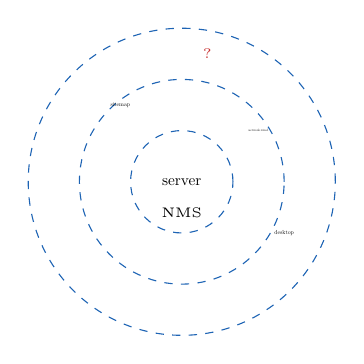
\begin{tikzpicture}[scale=0.65]
                    \node (nms) at (0, 0) {\iconserver[0.5cm]};
                    \node[font=\tiny] at (0, -0.6) {NMS};
                    \draw[tcpblue, dashed] (0, 0) circle (1);
                    \draw[tcpblue, dashed] (0, 0) circle (2);
                    \draw[tcpblue, dashed] (0, 0) circle (3);
                    \node at (1.5, 1) {\iconrouter[0.25cm]};
                    \node at (-1.2, 1.5) {\iconswitch[0.25cm]};
                    \node at (2, -1) {\iconpc[0.25cm]};
                    \node[font=\tiny, alertred] at (0.5, 2.5) {?};
                \end{tikzpicture}
            \end{center}
            \begin{block}{Discovery Protocols}
                \footnotesize
                ICMP (ping), ARP, SNMP, CDP/LLDP, DNS, NetBIOS
            \end{block}
        \end{column}
    \end{columns}
\end{frame}

% SLIDE 16: Network Discovery Methods
\begin{frame}{Network Discovery Methods}
    \begin{columns}[T]
        \begin{column}{0.48\textwidth}
            \begin{block}{Active Discovery}
                \footnotesize
                \textbf{Sends probes} to find devices:
                \begin{itemize}\setlength{\itemsep}{0pt}
                    \item Ping sweeps (ICMP)
                    \item Port scans (TCP/UDP)
                    \item SNMP queries
                    \item ARP requests
                \end{itemize}
                \textcolor{ogregreen}{\textbf{Pro}}: Comprehensive results\\
                \textcolor{alertred}{\textbf{Con}}: Generates traffic, may trigger alerts
            \end{block}
        \end{column}
        \begin{column}{0.48\textwidth}
            \begin{block}{Passive Discovery}
                \footnotesize
                \textbf{Listens} to existing traffic:
                \begin{itemize}\setlength{\itemsep}{0pt}
                    \item ARP table analysis
                    \item Switch MAC tables
                    \item Traffic sniffing
                    \item NetFlow/sFlow data
                \end{itemize}
                \textcolor{ogregreen}{\textbf{Pro}}: Stealthy, no extra traffic\\
                \textcolor{alertred}{\textbf{Con}}: Only sees active devices
            \end{block}
            \begin{alertblock}{Best Practice}
                \footnotesize
                Use \textbf{both methods}: Active for comprehensive scans, passive for continuous monitoring
            \end{alertblock}
        \end{column}
    \end{columns}
\end{frame}

% SLIDE 17: Nmap - The Network Mapper
\begin{frame}{Nmap --- The Network Mapper}
    \begin{columns}[T]
        \begin{column}{0.48\textwidth}
            \begin{block}{What is Nmap?}
                \footnotesize
                Open-source \textbf{network scanner} for:
                \begin{itemize}\setlength{\itemsep}{0pt}
                    \item Host discovery
                    \item Port scanning
                    \item Service/version detection
                    \item OS fingerprinting
                    \item Vulnerability scanning
                \end{itemize}
            \end{block}
            \begin{alertblock}{Legal Warning!}
                \footnotesize
                Only scan networks you \textbf{own} or have \textbf{written permission} to scan. Unauthorized scanning is illegal!
            \end{alertblock}
        \end{column}
        \begin{column}{0.48\textwidth}
            \begin{block}{Common Nmap Commands}
                \ttfamily\scriptsize
                \# Ping sweep (host discovery)\\
                nmap -sn 192.168.1.0/24\\[0.2em]
                \# SYN scan (stealth)\\
                nmap -sS 192.168.1.1\\[0.2em]
                \# Version detection\\
                nmap -sV 192.168.1.1\\[0.2em]
                \# OS detection\\
                nmap -O 192.168.1.1\\[0.2em]
                \# Aggressive scan\\
                nmap -A 192.168.1.1
            \end{block}
        \end{column}
    \end{columns}
\end{frame}

% SLIDE 18: Nmap Port Scanning Techniques
\begin{frame}{Nmap Port Scanning Techniques}
    \begin{columns}[T]
        \begin{column}{0.55\textwidth}
            \begin{block}{Scan Types Comparison}
                \footnotesize
                \begin{tabular}{@{}l c l c@{}}
                    \toprule
                    \textbf{Scan} & \textbf{Flag} & \textbf{Method} & \textbf{Stealth} \\
                    \midrule
                    TCP Connect & {-}sT & Full handshake & Low \\
                    SYN Scan & {-}sS & Half-open & Medium \\
                    UDP Scan & {-}sU & UDP probes & Medium \\
                    ACK Scan & {-}sA & Firewall map & High \\
                    FIN Scan & {-}sF & FIN flag only & High \\
                    \bottomrule
                \end{tabular}
            \end{block}
            \begin{exampleblock}{SYN Scan (Most Common)}
                \footnotesize
                Default for root/admin. Sends SYN, receives SYN-ACK (open) or RST (closed), then sends RST. Never completes connection!
            \end{exampleblock}
        \end{column}
        \begin{column}{0.42\textwidth}
            \begin{center}
                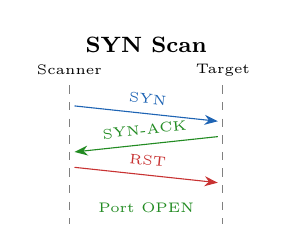
\begin{tikzpicture}[scale=0.65]
                    \node[font=\footnotesize] at (1.5, 4) {\textbf{SYN Scan}};
                    \node[font=\tiny] at (0, 3.5) {Scanner};
                    \node[font=\tiny] at (3, 3.5) {Target};
                    \draw[dashed, gray] (0, 3.2) -- (0, 0.5);
                    \draw[dashed, gray] (3, 3.2) -- (3, 0.5);
                    \draw[-{Stealth}, tcpblue] (0.1, 2.8) -- (2.9, 2.5) node[midway, above, font=\tiny, sloped] {SYN};
                    \draw[-{Stealth}, ogregreen] (2.9, 2.2) -- (0.1, 1.9) node[midway, above, font=\tiny, sloped] {SYN-ACK};
                    \draw[-{Stealth}, alertred] (0.1, 1.6) -- (2.9, 1.3) node[midway, above, font=\tiny, sloped] {RST};
                    \node[font=\tiny, ogregreen] at (1.5, 0.8) {Port OPEN};
                \end{tikzpicture}
            \end{center}
        \end{column}
    \end{columns}
\end{frame}

% SLIDE 19: Case Study - Puss in Boots' Reconnaissance
\begin{frame}{Case Study: Puss in Boots' Network Reconnaissance}
    \begin{alertblock}{``Fear Me, If You Dare!''}
        \footnotesize
        Puss in Boots has been hired as a security consultant to assess the Swamp Kingdom network. Shrek wants to know what devices are on the network and what services are exposed before the annual security audit.
        
        \vspace{0.2em}
        \textbf{Network information:}
        \begin{itemize}\setlength{\itemsep}{0pt}
            \item IP range: 10.0.0.0/16 (approximately 500 devices expected)
            \item Business hours: 9 AM -- 5 PM (critical operations)
            \item Shrek's requirement: ``Don't break anything!''
            \item Deadline: Full report needed within 48 hours
        \end{itemize}
        
        Puss needs to discover all hosts, identify open ports, and detect running services without disrupting the kingdom's operations.
    \end{alertblock}
    \begin{block}{Review Questions}
        \footnotesize
        1. What scan type for initial discovery? 2. How to minimize business impact? 3. What to document?
    \end{block}
\end{frame}

% SLIDE 20: Case Study Solution - Puss' Reconnaissance
\begin{frame}{Case Study Solution: Puss in Boots' Reconnaissance}
    \begin{exampleblock}{Solution: ``I Am Not a Kitten---I Am a Professional!''}
        \footnotesize
        \begin{enumerate}\setlength{\itemsep}{1pt}
            \item \textbf{Phase 1}: Ping sweep (-sn) during business hours---low impact discovery
            \item \textbf{Phase 2}: SYN scan (-sS) after hours---detailed port scanning
            \item \textbf{Phase 3}: Version detection (-sV) on critical services only
        \end{enumerate}
    \end{exampleblock}
    \begin{columns}[T]
        \begin{column}{0.48\textwidth}
            \begin{block}{Recommended Commands}
                \ttfamily\scriptsize
                \# Phase 1: Discovery (daytime)\\
                nmap -sn 10.0.0.0/16 -oN hosts.txt\\[0.2em]
                \# Phase 2: Port scan (night)\\
                nmap -sS -iL hosts.txt -oN ports.txt\\[0.2em]
                \# Phase 3: Services (targeted)\\
                nmap -sV -p 22,80,443 -iL critical.txt
            \end{block}
        \end{column}
        \begin{column}{0.48\textwidth}
            \begin{alertblock}{Key Lesson}
                \footnotesize
                Professional scanning is \textbf{staged and scheduled}. Balance thoroughness with business impact. Always document methodology and findings!
            \end{alertblock}
        \end{column}
    \end{columns}
\end{frame}

% SLIDE 21: Discovery Protocols (CDP, LLDP)
\begin{frame}{Discovery Protocols: CDP and LLDP}
    \begin{columns}[T]
        \begin{column}{0.48\textwidth}
            \begin{block}{CDP (Cisco Discovery Protocol)}
                \footnotesize
                \begin{itemize}\setlength{\itemsep}{0pt}
                    \item \textbf{Cisco proprietary}
                    \item Layer 2 multicast
                    \item 60-second advertisements
                    \item Shares: hostname, IP, platform, port ID
                \end{itemize}
                \ttfamily\scriptsize
                show cdp neighbors detail
            \end{block}
            \begin{block}{LLDP (Link Layer Discovery Protocol)}
                \footnotesize
                \begin{itemize}\setlength{\itemsep}{0pt}
                    \item \textbf{IEEE 802.1AB} (vendor-neutral)
                    \item Works across vendors
                    \item Similar info to CDP
                \end{itemize}
                \ttfamily\scriptsize
                show lldp neighbors detail
            \end{block}
        \end{column}
        \begin{column}{0.48\textwidth}
            \begin{center}
                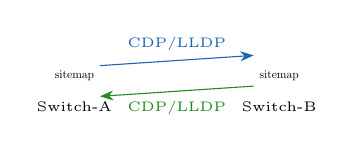
\begin{tikzpicture}[scale=0.65]
                    \node (sw1) at (0, 1.5) {\iconswitch[0.5cm]};
                    \node[font=\tiny] at (0, 0.9) {Switch-A};
                    \node (sw2) at (4, 1.5) {\iconswitch[0.5cm]};
                    \node[font=\tiny] at (4, 0.9) {Switch-B};
                    \draw[-{Stealth}, tcpblue] (0.5, 1.7) -- (3.5, 1.9) node[midway, above, font=\tiny] {CDP/LLDP};
                    \draw[-{Stealth}, ogregreen] (3.5, 1.3) -- (0.5, 1.1) node[midway, below, font=\tiny] {CDP/LLDP};
                \end{tikzpicture}
            \end{center}
            \begin{alertblock}{Security Warning}
                \footnotesize
                CDP/LLDP reveal network info to anyone connected. \textbf{Disable on edge ports} (user-facing, untrusted connections)!
            \end{alertblock}
        \end{column}
    \end{columns}
\end{frame}

% SLIDE 22: Performance Monitoring
\begin{frame}{Performance Monitoring}
    \begin{columns}[T]
        \begin{column}{0.48\textwidth}
            \begin{block}{What to Monitor}
                \footnotesize
                \begin{itemize}\setlength{\itemsep}{1pt}
                    \item \textbf{Bandwidth}: Link utilization \%
                    \item \textbf{Latency}: Round-trip time (ms)
                    \item \textbf{Jitter}: Latency variation
                    \item \textbf{Packet Loss}: \% dropped packets
                    \item \textbf{CPU}: Processor utilization
                    \item \textbf{Memory}: RAM usage
                \end{itemize}
            \end{block}
            \begin{exampleblock}{Monitoring Tools}
                \footnotesize
                PRTG, Nagios, Zabbix, LibreNMS, SolarWinds, Datadog
            \end{exampleblock}
        \end{column}
        \begin{column}{0.48\textwidth}
            \begin{block}{Performance Thresholds}
                \footnotesize
                \begin{tabular}{@{}l c c c@{}}
                    \toprule
                    \textbf{Metric} & \textbf{OK} & \textbf{Warn} & \textbf{Crit} \\
                    \midrule
                    CPU & $<$70\% & 70--85\% & $>$85\% \\
                    Memory & $<$75\% & 75--90\% & $>$90\% \\
                    Bandwidth & $<$60\% & 60--80\% & $>$80\% \\
                    Latency & $<$50ms & 50--100 & $>$100 \\
                    \bottomrule
                \end{tabular}
            \end{block}
            \begin{alertblock}{Baseline First!}
                \footnotesize
                Establish \textbf{normal} performance before setting alerts. What's ``high'' varies by environment.
            \end{alertblock}
        \end{column}
    \end{columns}
\end{frame}

% SLIDE 23: Availability Monitoring
\begin{frame}{Availability Monitoring}
    \begin{columns}[T]
        \begin{column}{0.48\textwidth}
            \begin{block}{Availability = Uptime}
                \footnotesize
                Measuring whether devices and services are \textbf{reachable and responding}:
                \begin{itemize}\setlength{\itemsep}{0pt}
                    \item Device reachability (is it up?)
                    \item Service availability (is it working?)
                    \item Response time (how fast?)
                \end{itemize}
            \end{block}
            \begin{block}{Monitoring Methods}
                \footnotesize
                \begin{tabular}{@{}l l c@{}}
                    \toprule
                    \textbf{Method} & \textbf{Tests} & \textbf{Freq} \\
                    \midrule
                    ICMP Ping & Reachability & 30--60s \\
                    TCP Check & Port response & 1--5 min \\
                    HTTP Check & Web service & 1--5 min \\
                    Synthetic & Full transaction & 5--15 min \\
                    \bottomrule
                \end{tabular}
            \end{block}
        \end{column}
        \begin{column}{0.48\textwidth}
            \begin{center}
                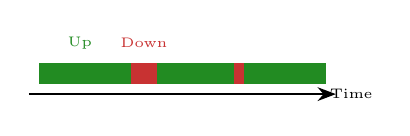
\begin{tikzpicture}[scale=0.65]
                    \draw[-{Stealth}, thick] (0, 0) -- (6, 0);
                    \node[font=\tiny] at (6.3, 0) {Time};
                    \fill[ogregreen] (0.2, 0.2) rectangle (2, 0.6);
                    \fill[ogregreen] (2.5, 0.2) rectangle (4, 0.6);
                    \fill[ogregreen] (4.2, 0.2) rectangle (5.8, 0.6);
                    \fill[alertred] (2, 0.2) rectangle (2.5, 0.6);
                    \fill[alertred] (4, 0.2) rectangle (4.2, 0.6);
                    \node[font=\tiny, ogregreen] at (1, 1) {Up};
                    \node[font=\tiny, alertred] at (2.25, 1) {Down};
                \end{tikzpicture}
            \end{center}
            \begin{alertblock}{Don't Just Ping!}
                \footnotesize
                A device can respond to ping but have \textbf{failed services}. Monitor what users actually use!
            \end{alertblock}
        \end{column}
    \end{columns}
\end{frame}

% SLIDE 24: Configuration Monitoring
\begin{frame}{Configuration Monitoring}
    \begin{columns}[T]
        \begin{column}{0.48\textwidth}
            \begin{block}{Purpose}
                \footnotesize
                Detect and alert on configuration changes:
                \begin{itemize}\setlength{\itemsep}{0pt}
                    \item \textbf{Unauthorized changes} (security)
                    \item \textbf{Drift from baseline} (compliance)
                    \item \textbf{Change verification} (operations)
                    \item \textbf{Audit trail} (governance)
                \end{itemize}
            \end{block}
            \begin{exampleblock}{Config Monitoring Tools}
                \footnotesize
                \textbf{RANCID}, \textbf{Oxidized}, SolarWinds NCM, Cisco Prime, Ansible
            \end{exampleblock}
        \end{column}
        \begin{column}{0.48\textwidth}
            \begin{center}
                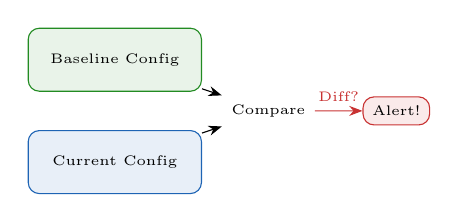
\begin{tikzpicture}[scale=0.65]
                    \node[draw=ogregreen, fill=ogregreen!10, rounded corners,
                          minimum width=2.2cm, minimum height=0.8cm, font=\tiny] 
                          (base) at (0, 2) {Baseline Config};
                    \node[draw=tcpblue, fill=tcpblue!10, rounded corners,
                          minimum width=2.2cm, minimum height=0.8cm, font=\tiny] 
                          (curr) at (0, 0) {Current Config};
                    \node[font=\tiny] (comp) at (3, 1) {Compare};
                    \draw[-{Stealth}] (base) -- (comp);
                    \draw[-{Stealth}] (curr) -- (comp);
                    \node[draw=alertred, fill=alertred!10, rounded corners, font=\tiny] (alert) at (5.5, 1) {Alert!};
                    \draw[-{Stealth}, alertred] (comp) -- node[above, font=\tiny] {Diff?} (alert);
                \end{tikzpicture}
            \end{center}
            \begin{block}{What Triggers Alerts}
                \footnotesize
                Any config change, specific keywords (passwords, ACLs), deviation from template, unauthorized user
            \end{block}
        \end{column}
    \end{columns}
\end{frame}

% SLIDE 25: SNMP Overview
\begin{frame}{Section 8.3: SNMP --- Simple Network Management Protocol}
    \begin{columns}[T]
        \begin{column}{0.48\textwidth}
            \begin{block}{What is SNMP?}
                \footnotesize
                The \textbf{standard protocol} for network device monitoring and management:
                \begin{itemize}\setlength{\itemsep}{0pt}
                    \item Query device statistics
                    \item Receive alerts (traps)
                    \item Configure devices remotely
                    \item Works across vendors
                \end{itemize}
            \end{block}
            \begin{block}{Key SNMP Terms}
                \footnotesize
                \textbf{Agent}: Software on managed device; \textbf{Manager/NMS}: Central monitoring station; \textbf{MIB}: Management Information Base; \textbf{OID}: Object Identifier; \textbf{Community}: Authentication string
            \end{block}
        \end{column}
        \begin{column}{0.48\textwidth}
            \begin{center}
                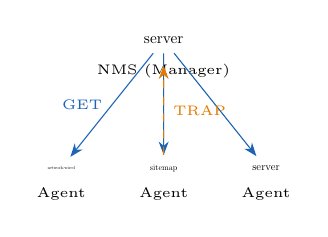
\begin{tikzpicture}[scale=0.65]
                    \node (nms) at (2, 3) {\iconserver[0.5cm]};
                    \node[font=\tiny] at (2, 2.4) {NMS (Manager)};
                    \node (r1) at (0, 0.5) {\iconrouter[0.35cm]};
                    \node[font=\tiny] at (0, 0) {Agent};
                    \node (sw1) at (2, 0.5) {\iconswitch[0.35cm]};
                    \node[font=\tiny] at (2, 0) {Agent};
                    \node (s1) at (4, 0.5) {\iconserver[0.35cm]};
                    \node[font=\tiny] at (4, 0) {Agent};
                    \draw[-{Stealth}, tcpblue] (nms) -- (r1) node[midway, left, font=\tiny] {GET};
                    \draw[-{Stealth}, tcpblue] (nms) -- (sw1);
                    \draw[-{Stealth}, tcpblue] (nms) -- (s1);
                    \draw[-{Stealth}, aborange, dashed] (sw1) -- (2, 2.5) node[midway, right, font=\tiny] {TRAP};
                \end{tikzpicture}
            \end{center}
            \begin{block}{SNMP Ports}
                \footnotesize
                \textbf{UDP 161}: Agent (queries); \textbf{UDP 162}: Manager (traps)
            \end{block}
        \end{column}
    \end{columns}
\end{frame}

% SLIDE 26: SNMP Operations
\begin{frame}{SNMP Operations}
    \begin{columns}[T]
        \begin{column}{0.48\textwidth}
            \begin{block}{SNMP Operations}
                \footnotesize
                \begin{tabular}{@{}l l l@{}}
                    \toprule
                    \textbf{Operation} & \textbf{Direction} & \textbf{Purpose} \\
                    \midrule
                    GET & Mgr to Agent & Read value \\
                    GET-NEXT & Mgr to Agent & Walk MIB \\
                    GET-BULK & Mgr to Agent & Read many \\
                    SET & Mgr to Agent & Write value \\
                    TRAP & Agent to Mgr & Alert (async) \\
                    INFORM & Agent to Mgr & Ack'd trap \\
                    \bottomrule
                \end{tabular}
            \end{block}
            \begin{exampleblock}{Polling vs Traps}
                \footnotesize
                \textbf{Polling}: NMS regularly queries (GET)\\
                \textbf{Traps}: Agent sends alerts immediately
            \end{exampleblock}
        \end{column}
        \begin{column}{0.48\textwidth}
            \begin{center}
                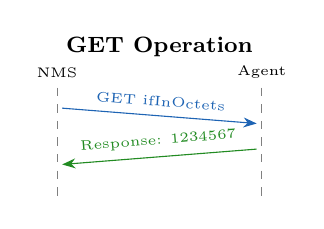
\begin{tikzpicture}[scale=0.65]
                    \node[font=\footnotesize] at (2, 3.5) {\textbf{GET Operation}};
                    \node[font=\tiny] at (0, 3) {NMS};
                    \node[font=\tiny] at (4, 3) {Agent};
                    \draw[dashed, gray] (0, 2.7) -- (0, 0.5);
                    \draw[dashed, gray] (4, 2.7) -- (4, 0.5);
                    \draw[-{Stealth}, tcpblue] (0.1, 2.3) -- (3.9, 2) node[midway, above, font=\tiny, sloped] {GET ifInOctets};
                    \draw[-{Stealth}, ogregreen] (3.9, 1.5) -- (0.1, 1.2) node[midway, above, font=\tiny, sloped] {Response: 1234567};
                \end{tikzpicture}
            \end{center}
            \begin{block}{Common OIDs}
                \ttfamily\scriptsize
                .1.3.6.1.2.1.1.1 = sysDescr\\
                .1.3.6.1.2.1.1.3 = sysUpTime\\
                .1.3.6.1.2.1.2.2 = ifTable
            \end{block}
        \end{column}
    \end{columns}
\end{frame}

% SLIDE 27: SNMP Versions and Security
\begin{frame}{SNMP Versions and Security}
    \begin{columns}[T]
        \begin{column}{0.55\textwidth}
            \begin{block}{SNMP Version Comparison}
                \footnotesize
                \begin{tabular}{@{}l c c c@{}}
                    \toprule
                    \textbf{Feature} & \textbf{v1} & \textbf{v2c} & \textbf{v3} \\
                    \midrule
                    Authentication & Community & Community & User/Pass \\
                    Encryption & None & None & AES/DES \\
                    Integrity & None & None & MD5/SHA \\
                    GET-BULK & No & Yes & Yes \\
                    Security & \textcolor{alertred}{Low} & \textcolor{alertred}{Low} & \textcolor{ogregreen}{High} \\
                    \bottomrule
                \end{tabular}
            \end{block}
            \begin{alertblock}{Critical Security Issue!}
                \footnotesize
                SNMPv1/v2c send community strings in \textbf{cleartext}! Anyone sniffing traffic can capture them.
            \end{alertblock}
        \end{column}
        \begin{column}{0.42\textwidth}
            \begin{block}{SNMPv3 Security Levels}
                \footnotesize
                \begin{itemize}\setlength{\itemsep}{1pt}
                    \item \textbf{noAuthNoPriv}: Username only
                    \item \textbf{authNoPriv}: + Authentication
                    \item \textbf{authPriv}: + Encryption
                \end{itemize}
            \end{block}
            \begin{exampleblock}{Exam Tip}
                \footnotesize
                SNMPv3 = \textbf{A}uthentication + \textbf{E}ncryption + \textbf{I}ntegrity. Always prefer v3 for production!
            \end{exampleblock}
        \end{column}
    \end{columns}
\end{frame}

% SLIDE 28: Case Study - Lord Farquaad's SNMP Disaster
\begin{frame}{Case Study: Lord Farquaad's SNMP Disaster}
    \begin{alertblock}{``Some of You May Be Compromised...''}
        \footnotesize
        Lord Farquaad's IT team configured SNMP on all Duloc network devices using community strings ``public'' (read-only) and ``private'' (read-write). They thought these were just examples from the documentation.
        
        \vspace{0.2em}
        A security audit reveals:
        \begin{itemize}\setlength{\itemsep}{0pt}
            \item Attackers have been querying device configs for weeks
            \item Someone changed the ACLs on the border router
            \item Wireshark capture shows SNMP traffic with ``public'' in cleartext
            \item All 50 network devices use identical community strings
        \end{itemize}
        
        \textbf{Evidence}: \texttt{snmpwalk -v2c -c public 10.0.0.1}
    \end{alertblock}
    \begin{block}{Review Questions}
        \footnotesize
        1. What SNMP vulnerabilities were exploited? 2. What version should they migrate to? 3. What immediate steps are needed?
    \end{block}
\end{frame}

% SLIDE 29: Case Study Solution - Farquaad's SNMP
\begin{frame}{Case Study Solution: Lord Farquaad's SNMP Disaster}
    \begin{exampleblock}{Solution: ``This Is Not the Fairy Tale I Wanted!''}
        \footnotesize
        \begin{enumerate}\setlength{\itemsep}{1pt}
            \item \textbf{Vulnerabilities}: Default community strings + cleartext transmission (v2c) + RW access
            \item \textbf{Migration}: Upgrade to \textbf{SNMPv3} with authPriv (authentication + encryption)
            \item \textbf{Immediate}: Change all communities, implement ACLs, audit all configs, disable write where not needed
        \end{enumerate}
    \end{exampleblock}
    \begin{columns}[T]
        \begin{column}{0.48\textwidth}
            \begin{center}
                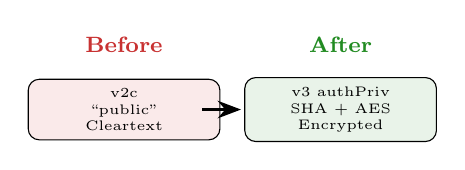
\begin{tikzpicture}[scale=0.55]
                    \node[font=\footnotesize, alertred] at (0, 3) {\textbf{Before}};
                    \node[draw, fill=alertred!10, rounded corners, font=\tiny, text width=2.2cm, align=center] at (0, 1.5) {v2c\\``public''\\Cleartext};
                    \node[font=\footnotesize, ogregreen] at (5, 3) {\textbf{After}};
                    \node[draw, fill=ogregreen!10, rounded corners, font=\tiny, text width=2.2cm, align=center] at (5, 1.5) {v3 authPriv\\SHA + AES\\Encrypted};
                    \draw[-{Stealth}, very thick] (1.8, 1.5) -- (2.7, 1.5);
                \end{tikzpicture}
            \end{center}
        \end{column}
        \begin{column}{0.48\textwidth}
            \begin{alertblock}{Key Lessons}
                \footnotesize
                Never use default credentials; v1/v2c = cleartext = vulnerable; limit SNMP access with ACLs; disable write access unless needed
            \end{alertblock}
        \end{column}
    \end{columns}
\end{frame}

% SLIDE 30: Event Management & Logging
\begin{frame}{Section 8.4: Event Management \& Logging}
    \begin{columns}[T]
        \begin{column}{0.48\textwidth}
            \begin{block}{Why Logging Matters}
                \footnotesize
                \begin{itemize}\setlength{\itemsep}{1pt}
                    \item \textbf{Troubleshooting}: What happened when?
                    \item \textbf{Security}: Detect breaches and attacks
                    \item \textbf{Compliance}: Audit requirements
                    \item \textbf{Capacity}: Trend analysis
                    \item \textbf{Accountability}: Who did what?
                \end{itemize}
            \end{block}
            \begin{alertblock}{Key Principle}
                \footnotesize
                If it's not logged, it didn't happen! Centralize logs for correlation and retention.
            \end{alertblock}
        \end{column}
        \begin{column}{0.48\textwidth}
            \begin{center}
                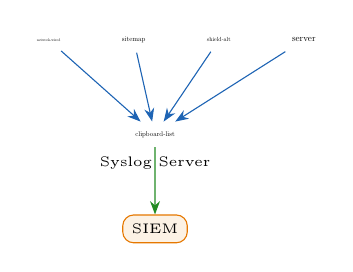
\begin{tikzpicture}[scale=0.6]
                    \node (r1) at (0, 3) {\iconrouter[0.3cm]};
                    \node (sw1) at (1.8, 3) {\iconswitch[0.3cm]};
                    \node (fw1) at (3.6, 3) {\iconfirewall[0.3cm]};
                    \node (s1) at (5.4, 3) {\iconserver[0.3cm]};
                    \node (syslog) at (2.25, 1) {\iconlog[0.5cm]};
                    \node[font=\tiny] at (2.25, 0.4) {Syslog Server};
                    \node[draw=aborange, fill=aborange!10, rounded corners, font=\tiny] (siem) at (2.25, -1) {SIEM};
                    \draw[-{Stealth}, tcpblue] (r1) -- (syslog);
                    \draw[-{Stealth}, tcpblue] (sw1) -- (syslog);
                    \draw[-{Stealth}, tcpblue] (fw1) -- (syslog);
                    \draw[-{Stealth}, tcpblue] (s1) -- (syslog);
                    \draw[-{Stealth}, ogregreen] (syslog) -- (siem);
                \end{tikzpicture}
            \end{center}
            \begin{block}{Log Flow}
                \footnotesize
                Devices $\rightarrow$ Syslog Server $\rightarrow$ SIEM $\rightarrow$ Alerts/Dashboards
            \end{block}
        \end{column}
    \end{columns}
\end{frame}

% SLIDE 31: Syslog Protocol and Severity Levels
\begin{frame}{Syslog Protocol and Severity Levels}
    \begin{columns}[T]
        \begin{column}{0.48\textwidth}
            \begin{block}{Syslog Basics}
                \footnotesize
                \begin{itemize}\setlength{\itemsep}{0pt}
                    \item Standard logging protocol
                    \item \textbf{UDP 514} (traditional)
                    \item \textbf{TCP 514} (reliable)
                    \item \textbf{TCP 6514} (TLS encrypted)
                \end{itemize}
            \end{block}
            \begin{exampleblock}{Syslog Message Format}
                \ttfamily\scriptsize
                <priority>timestamp host message\\[0.2em]
                <134>Jan 25 10:30:15 router1\\
                \%LINK-3-UPDOWN: Interface\\
                Gi0/1 changed state to down
            \end{exampleblock}
        \end{column}
        \begin{column}{0.48\textwidth}
            \begin{block}{Severity Levels (Memorize!)}
                \scriptsize
                \begin{tabular}{@{}c l l@{}}
                    \toprule
                    \textbf{Level} & \textbf{Name} & \textbf{Description} \\
                    \midrule
                    0 & Emergency & System unusable \\
                    1 & Alert & Immediate action \\
                    2 & Critical & Critical condition \\
                    3 & Error & Error condition \\
                    4 & Warning & Warning condition \\
                    5 & Notice & Normal but notable \\
                    6 & Info & Informational \\
                    7 & Debug & Debug messages \\
                    \bottomrule
                \end{tabular}
            \end{block}
        \end{column}
    \end{columns}
\end{frame}

% SLIDE 32: SIEM
\begin{frame}{SIEM --- Security Information and Event Management}
    \begin{columns}[T]
        \begin{column}{0.48\textwidth}
            \begin{block}{What is SIEM?}
                \footnotesize
                Central platform that:
                \begin{itemize}\setlength{\itemsep}{0pt}
                    \item \textbf{Aggregates} logs from all sources
                    \item \textbf{Normalizes} different log formats
                    \item \textbf{Correlates} events across systems
                    \item \textbf{Analyzes} for patterns/threats
                    \item \textbf{Alerts} on suspicious activity
                    \item \textbf{Reports} for compliance
                \end{itemize}
            \end{block}
            \begin{exampleblock}{Popular SIEM Platforms}
                \footnotesize
                Splunk, IBM QRadar, Microsoft Sentinel, Elastic SIEM, AlienVault
            \end{exampleblock}
        \end{column}
        \begin{column}{0.48\textwidth}
            \begin{center}
                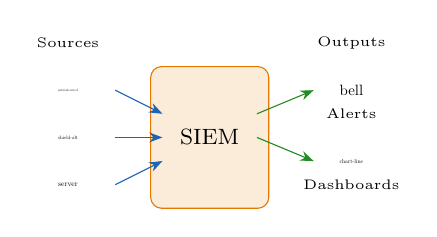
\begin{tikzpicture}[scale=0.6]
                    \node[font=\tiny] at (-1, 3.5) {Sources};
                    \node at (-1, 2.5) {\iconrouter[0.25cm]};
                    \node at (-1, 1.5) {\iconfirewall[0.25cm]};
                    \node at (-1, 0.5) {\iconserver[0.25cm]};
                    \node[draw=aborange, fill=aborange!15, rounded corners, minimum width=1.5cm, minimum height=1.8cm, font=\footnotesize] (siem) at (2, 1.5) {SIEM};
                    \node[font=\tiny] at (5, 3.5) {Outputs};
                    \node at (5, 2.5) {\iconalert[0.3cm]};
                    \node[font=\tiny] at (5, 2) {Alerts};
                    \node at (5, 1) {\iconchart[0.3cm]};
                    \node[font=\tiny] at (5, 0.5) {Dashboards};
                    \draw[-{Stealth}, tcpblue] (0, 2.5) -- (1, 2);
                    \draw[-{Stealth}, tcpblue] (0, 1.5) -- (1, 1.5);
                    \draw[-{Stealth}, tcpblue] (0, 0.5) -- (1, 1);
                    \draw[-{Stealth}, ogregreen] (3, 2) -- (4.2, 2.5);
                    \draw[-{Stealth}, ogregreen] (3, 1.5) -- (4.2, 1);
                \end{tikzpicture}
            \end{center}
            \begin{block}{Correlation Example}
                \footnotesize
                Failed logins (Server) + Port scan (Firewall) + New admin (AD) = Possible breach!
            \end{block}
        \end{column}
    \end{columns}
\end{frame}

% SLIDE 33: Log Reviews and Alert Prioritization
\begin{frame}{Log Reviews and Alert Prioritization}
    \begin{columns}[T]
        \begin{column}{0.48\textwidth}
            \begin{block}{Alert Priority Matrix}
                \footnotesize
                \begin{tabular}{@{}l c l@{}}
                    \toprule
                    \textbf{Priority} & \textbf{Response} & \textbf{Example} \\
                    \midrule
                    P1 Critical & 15 min & Security breach \\
                    P2 High & 1 hour & Service outage \\
                    P3 Medium & 4 hours & Degraded perf \\
                    P4 Low & Next day & Minor warning \\
                    \bottomrule
                \end{tabular}
            \end{block}
            \begin{block}{Review Schedule}
                \footnotesize
                \textbf{Real-time}: P1/P2 alerts; \textbf{Daily}: Security events; \textbf{Weekly}: Trend analysis; \textbf{Monthly}: Compliance reports
            \end{block}
        \end{column}
        \begin{column}{0.48\textwidth}
            \begin{alertblock}{Alert Fatigue is Real!}
                \footnotesize
                Too many alerts = ignored alerts. Tune thresholds to reduce noise:
                \begin{itemize}\setlength{\itemsep}{0pt}
                    \item Suppress known false positives
                    \item Group related events
                    \item Set appropriate thresholds
                    \item Regularly review and tune rules
                \end{itemize}
            \end{alertblock}
            \begin{exampleblock}{Good Alert Design}
                \footnotesize
                \textbf{Actionable}: Clear what to do; \textbf{Contextual}: Includes relevant info; \textbf{Prioritized}: Severity is accurate
            \end{exampleblock}
        \end{column}
    \end{columns}
\end{frame}

% SLIDE 34: Packet Capture and Analysis
\begin{frame}{Section 8.5: Packet Capture and Analysis}
    \begin{columns}[T]
        \begin{column}{0.48\textwidth}
            \begin{block}{Why Capture Packets?}
                \footnotesize
                \begin{itemize}\setlength{\itemsep}{1pt}
                    \item \textbf{Troubleshooting}: See actual traffic
                    \item \textbf{Security}: Detect malicious activity
                    \item \textbf{Performance}: Analyze latency issues
                    \item \textbf{Learning}: Understand protocols
                    \item \textbf{Forensics}: Incident investigation
                \end{itemize}
            \end{block}
            \begin{block}{Capture Methods}
                \footnotesize
                \textbf{SPAN/Mirror Port}: Switch copies traffic; \textbf{Network TAP}: Hardware inline device; \textbf{Host-based}: Capture on endpoint
            \end{block}
        \end{column}
        \begin{column}{0.48\textwidth}
            \begin{center}
                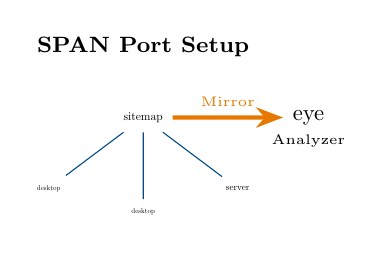
\begin{tikzpicture}[scale=0.6]
                    \node[font=\footnotesize] at (2, 4) {\textbf{SPAN Port Setup}};
                    \node (sw) at (2, 2.5) {\iconswitch[0.5cm]};
                    \node (pc1) at (0, 1) {\iconpc[0.3cm]};
                    \node (pc2) at (2, 0.5) {\iconpc[0.3cm]};
                    \node (srv) at (4, 1) {\iconserver[0.3cm]};
                    \node (analyzer) at (5.5, 2.5) {\iconeye[0.4cm]};
                    \node[font=\tiny] at (5.5, 2) {Analyzer};
                    \draw[rctcblue] (pc1) -- (sw);
                    \draw[rctcblue] (pc2) -- (sw);
                    \draw[rctcblue] (srv) -- (sw);
                    \draw[-{Stealth}, aborange, line width=1.5pt] (sw) -- (analyzer) node[midway, above, font=\tiny] {Mirror};
                \end{tikzpicture}
            \end{center}
            \begin{block}{Key Tools}
                \footnotesize
                \textbf{tcpdump}: CLI packet capture; \textbf{Wireshark}: GUI protocol analyzer; \textbf{tshark}: Wireshark CLI version
            \end{block}
        \end{column}
    \end{columns}
\end{frame}

% SLIDE 35: tcpdump and Wireshark
\begin{frame}{tcpdump and Wireshark}
    \begin{columns}[T]
        \begin{column}{0.48\textwidth}
            \begin{block}{tcpdump (Command Line)}
                \ttfamily\scriptsize
                \# Capture on interface\\
                tcpdump -i eth0\\[0.2em]
                \# Write to file\\
                tcpdump -w capture.pcap\\[0.2em]
                \# Filter by port\\
                tcpdump port 80\\[0.2em]
                \# Filter by host\\
                tcpdump host 10.0.0.1\\[0.2em]
                \# Combine filters\\
                tcpdump -i eth0 host 10.0.0.1 and port 443
            \end{block}
        \end{column}
        \begin{column}{0.48\textwidth}
            \begin{block}{Wireshark (GUI)}
                \footnotesize
                Full protocol analyzer with packet list, details, bytes views; follow TCP/UDP streams; expert analysis
            \end{block}
            \begin{block}{Wireshark Display Filters}
                \ttfamily\scriptsize
                ip.addr == 10.0.0.1\\
                tcp.port == 443\\
                http.request\\
                dns.qry.name contains "google"\\
                tcp.flags.syn == 1
            \end{block}
            \begin{alertblock}{Capture vs Display Filters}
                \footnotesize
                \textbf{Capture filters}: Applied during capture (tcpdump syntax) --- \texttt{host 10.0.0.1}\\
                \textbf{Display filters}: Applied after capture (Wireshark syntax) --- \texttt{ip.addr == 10.0.0.1}
            \end{alertblock}
        \end{column}
    \end{columns}
\end{frame}

% SLIDE 36: Case Study - Fiona's Network Mystery
\begin{frame}{Case Study: Princess Fiona's Network Mystery}
    \begin{alertblock}{``By Day One Way, By Night Another...''}
        \footnotesize
        Princess Fiona notices the Far Far Away Castle network becomes extremely slow every afternoon around 3 PM. Users complain about timeouts, dropped connections, and slow file transfers.
        
        \vspace{0.2em}
        Basic monitoring shows:
        \begin{itemize}\setlength{\itemsep}{0pt}
            \item Core switch uplink hits 95\% utilization at 3 PM
            \item CPU and memory on all devices are normal
            \item No errors or discards on interfaces
            \item Problem resolves itself by 5 PM
        \end{itemize}
        
        \textbf{Available tools}: Wireshark laptop, SPAN port access on core switch
        
        Fiona needs to identify what's consuming all the bandwidth!
    \end{alertblock}
    \begin{block}{Review Questions}
        \footnotesize
        1. How should Fiona configure packet capture? 2. What Wireshark features help? 3. What metrics to analyze?
    \end{block}
\end{frame}

% SLIDE 37: Case Study Solution - Fiona's Mystery
\begin{frame}{Case Study Solution: Princess Fiona's Network Mystery}
    \begin{exampleblock}{Solution: ``Better Out Than In!''}
        \footnotesize
        \begin{enumerate}\setlength{\itemsep}{1pt}
            \item Configure SPAN to mirror uplink traffic to analyzer laptop during peak time
            \item Use Wireshark \textbf{Statistics $\rightarrow$ Conversations} and \textbf{Endpoints} to find top talkers
            \item Analyze: bytes by host, protocol distribution, conversation statistics
        \end{enumerate}
    \end{exampleblock}
    \begin{columns}[T]
        \begin{column}{0.48\textwidth}
            \begin{block}{Discovery}
                \footnotesize
                Wireshark revealed:
                \begin{itemize}\setlength{\itemsep}{0pt}
                    \item Backup server $\rightarrow$ Cloud storage
                    \item 500+ Mbps sustained transfer
                    \item Scheduled backup job at 3 PM
                    \item Runs during business hours!
                \end{itemize}
            \end{block}
        \end{column}
        \begin{column}{0.48\textwidth}
            \begin{block}{Resolution}
                \footnotesize
                Reschedule backups to 2 AM; implement QoS for backup traffic; add bandwidth monitoring alerts
            \end{block}
            \begin{alertblock}{Key Lesson}
                \footnotesize
                Packet capture reveals what dashboards miss. \textbf{Statistics $\rightarrow$ Endpoints} is your friend!
            \end{alertblock}
        \end{column}
    \end{columns}
\end{frame}

% SLIDE 38: Traffic Monitoring & Flow Data
\begin{frame}{Section 8.6: Traffic Monitoring \& Flow Data}
    \begin{columns}[T]
        \begin{column}{0.48\textwidth}
            \begin{block}{Flow Data vs Packet Capture}
                \footnotesize
                \begin{tabular}{@{}l l l@{}}
                    \toprule
                    & \textbf{Flow} & \textbf{Packet} \\
                    \midrule
                    Content & Metadata & Full data \\
                    Storage & Low & High \\
                    Privacy & Better & Sensitive \\
                    Detail & Summary & Complete \\
                    Use & Trends & Deep dive \\
                    \bottomrule
                \end{tabular}
            \end{block}
            \begin{block}{Flow = Conversation Summary}
                \footnotesize
                Source IP, Dest IP, Ports, Protocol, Bytes, Packets, Duration, Timestamps
            \end{block}
        \end{column}
        \begin{column}{0.48\textwidth}
            \begin{center}
                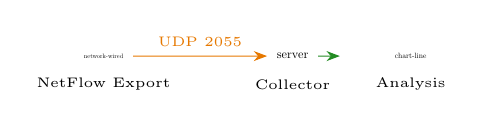
\begin{tikzpicture}[scale=0.6]
                    \node (router) at (0, 2) {\iconrouter[0.5cm]};
                    \node[font=\tiny] at (0, 1.4) {NetFlow Export};
                    \node (collector) at (4, 2) {\iconserver[0.4cm]};
                    \node[font=\tiny] at (4, 1.4) {Collector};
                    \node at (6.5, 2) {\iconchart[0.4cm]};
                    \node[font=\tiny] at (6.5, 1.4) {Analysis};
                    \draw[-{Stealth}, aborange] (router) -- (collector) node[midway, above, font=\tiny] {UDP 2055};
                    \draw[-{Stealth}, ogregreen] (collector) -- (5, 2);
                \end{tikzpicture}
            \end{center}
            
            \begin{block}{Flow Protocols}
                \footnotesize
                \begin{tabular}{@{}l l c@{}}
                    \toprule
                    \textbf{Protocol} & \textbf{Vendor} & \textbf{Port} \\
                    \midrule
                    NetFlow & Cisco & UDP 2055 \\
                    sFlow & Multi & UDP 6343 \\
                    IPFIX & Standard & UDP 4739 \\
                    J-Flow & Juniper & UDP 2055 \\
                    \bottomrule
                \end{tabular}
            \end{block}
        \end{column}
    \end{columns}
\end{frame}

% SLIDE 39: QoS and Traffic Shaping
\begin{frame}{QoS and Traffic Shaping}
    \begin{columns}[T]
        \begin{column}{0.48\textwidth}
            \begin{block}{QoS Purpose}
                \footnotesize
                Prioritize critical traffic when bandwidth is limited:
                \begin{itemize}\setlength{\itemsep}{0pt}
                    \item Voice/video over bulk data
                    \item Business apps over social media
                    \item Guaranteed bandwidth for critical systems
                \end{itemize}
            \end{block}
            \begin{block}{DSCP Values (Review)}
                \footnotesize
                \begin{tabular}{@{}l c l@{}}
                    \toprule
                    \textbf{Class} & \textbf{DSCP} & \textbf{Use} \\
                    \midrule
                    EF & 46 & Voice \\
                    AF41 & 34 & Video \\
                    AF21 & 18 & Critical data \\
                    BE & 0 & Default \\
                    \bottomrule
                \end{tabular}
            \end{block}
        \end{column}
        \begin{column}{0.48\textwidth}
            \begin{block}{Policing vs Shaping}
                \footnotesize
                \textbf{Policing}: Drop excess traffic immediately (hard limit, can cause packet loss)
                
                \vspace{0.2em}
                \textbf{Shaping}: Buffer and delay excess traffic (smoother flow, adds latency)
            \end{block}
            \begin{alertblock}{QoS Only Helps When...}
                \footnotesize
                There's \textbf{congestion}! QoS doesn't add bandwidth---it manages limited bandwidth intelligently.
            \end{alertblock}
        \end{column}
    \end{columns}
\end{frame}

% SLIDE 40: Module Summary
\begin{frame}{Module 8 Summary and Key Takeaways}
    \begin{columns}[T]
        \begin{column}{0.48\textwidth}
            \begin{block}{Documentation \& Policies}
                \footnotesize
                \begin{itemize}\setlength{\itemsep}{0pt}
                    \item \textbf{Change management}: Request $\rightarrow$ Review $\rightarrow$ Approve $\rightarrow$ Implement
                    \item \textbf{Physical diagrams}: Where things are
                    \item \textbf{Logical diagrams}: How things connect
                    \item \textbf{IPAM}: Track all IP allocations
                \end{itemize}
            \end{block}
            \begin{block}{Monitoring \& Analysis}
                \footnotesize
                \begin{itemize}\setlength{\itemsep}{0pt}
                    \item \textbf{SNMP}: v3 for security (auth + encryption)
                    \item \textbf{Syslog}: Levels 0--7 (Emergency to Debug)
                    \item \textbf{Packet capture}: tcpdump, Wireshark
                    \item \textbf{Flow data}: NetFlow, sFlow, IPFIX
                \end{itemize}
            \end{block}
        \end{column}
        \begin{column}{0.48\textwidth}
            \begin{block}{Key Ports Reference}
                \footnotesize
                \begin{tabular}{@{}l c l@{}}
                    \toprule
                    \textbf{Protocol} & \textbf{Port} & \textbf{Purpose} \\
                    \midrule
                    SNMP & UDP 161 & Agent queries \\
                    SNMP Trap & UDP 162 & Alerts \\
                    Syslog & UDP 514 & Logging \\
                    Syslog TLS & TCP 6514 & Secure logs \\
                    NetFlow & UDP 2055 & Flow export \\
                    sFlow & UDP 6343 & Flow export \\
                    \bottomrule
                \end{tabular}
            \end{block}
            \begin{alertblock}{Exam Reminders}
                \footnotesize
                Syslog 0 = Emergency, 7 = Debug; SNMPv3 = auth + encryption; SPAN/mirror for packet capture
            \end{alertblock}
        \end{column}
    \end{columns}
\end{frame}

\end{document}
